% status: 0
% chapter: Virtual Machines
% 
\title{RESTful API service to enable ease of portability of virtual
machines leveraging libcloud/boto}


\author{Harshad Pitkar}
\affiliation{%
  \institution{Indiana University}
  \city{Bloomington} 
  \state{IN} 
  \postcode{47408}
  \country{USA}}
\email{hpitkar@iu.edu}

\author{Sushant Athaley}
\affiliation{%
  \institution{Indiana University}
  \streetaddress{Smith Research Center}
  \city{Bloomington} 
  \state{IN} 
  \postcode{47408}
  \country{USA}}
\email{sathaley@iu.edu}

\author{Michael Robinson}
\affiliation{%
  \institution{Indiana University}
  \city{Bloomington} 
  \state{IN} 
  \postcode{47408}
  \country{USA}}
\email{micbrobi@iu.edu}


% The default list of authors is too long for headers}
\renewcommand{\shortauthors}{H. Pitkar, S. Athaley, M. Robinson}


\begin{abstract}
Our research measures how the portability of an application is impacted by decisions 
made early in the software lifecycle when native cloud provider APIs are used. We  
demonstrate how efforts to leverage scalable, reproducable solutions like boto and 
libcloud are advantageous. We derived reproducable code using Swagger and Python
to show how libraries like boto and libcloud can be used to migrate an application from 
one cloud provider to another with a measurable reduction in human error and with less 
time to execute. Additionally, we leveraged Swagger to develop RESTful APIs to 
further improve the gains. We captured the results of the research to share the derived 
code and concluded how the research can be applied to existing and new development efforts 
intending to leverage cloud providers. 
\end{abstract}

\keywords{hid-sp18-518, hid-sp18-517, hid-sp18-402, libcloud, boto}


\maketitle

\section{Introduction}\label{introduction}

Cloud portability is a growing area of research due to the increased profiliferation of 
cloud providers~\cite{hid-sp18-518-Cloud-Council}. Each provider has unique APIs and 
tools to their cloud environments  which can disincentivize portability as it influences 
a consumer to  stay with their existing solution provider. Efforts to standardize 
cloud portability like TOSCA have made progress yet participation by cloud providers is 
constrained due to the competitive nature in the  space. Each cloud provider is looking 
to retain their userbase and there is also a desire by each provider to become the de 
facto  standard by being the market leader. To fill the gap, solutions like Apache 
libcloud and boto have delivered an abstraction solution to developers to design 
applications that are easy to port.

Developers are already confronted with a lack of transparency on which cloud provider is 
optimal for the long-term sustainability of their application. Additionally, attempts to 
abstract away from cloud providers are helpful yet their non-standardization still 
potentially locks you into the solutions provided by Apache or communities like boto. We 
will deliver a continuation of that abstraction concept with an accepted standard, REST, 
to extend libcloud and boto. By leveraging REST, we intend to introduce a standardized 
implementation that leverages cloud portability libraries to manage the diversity of 
cloud applications. A high-level abstract of the concept is shown in Figure~\ref{F:arch}.

\begin{figure}[!ht]
  \centering
  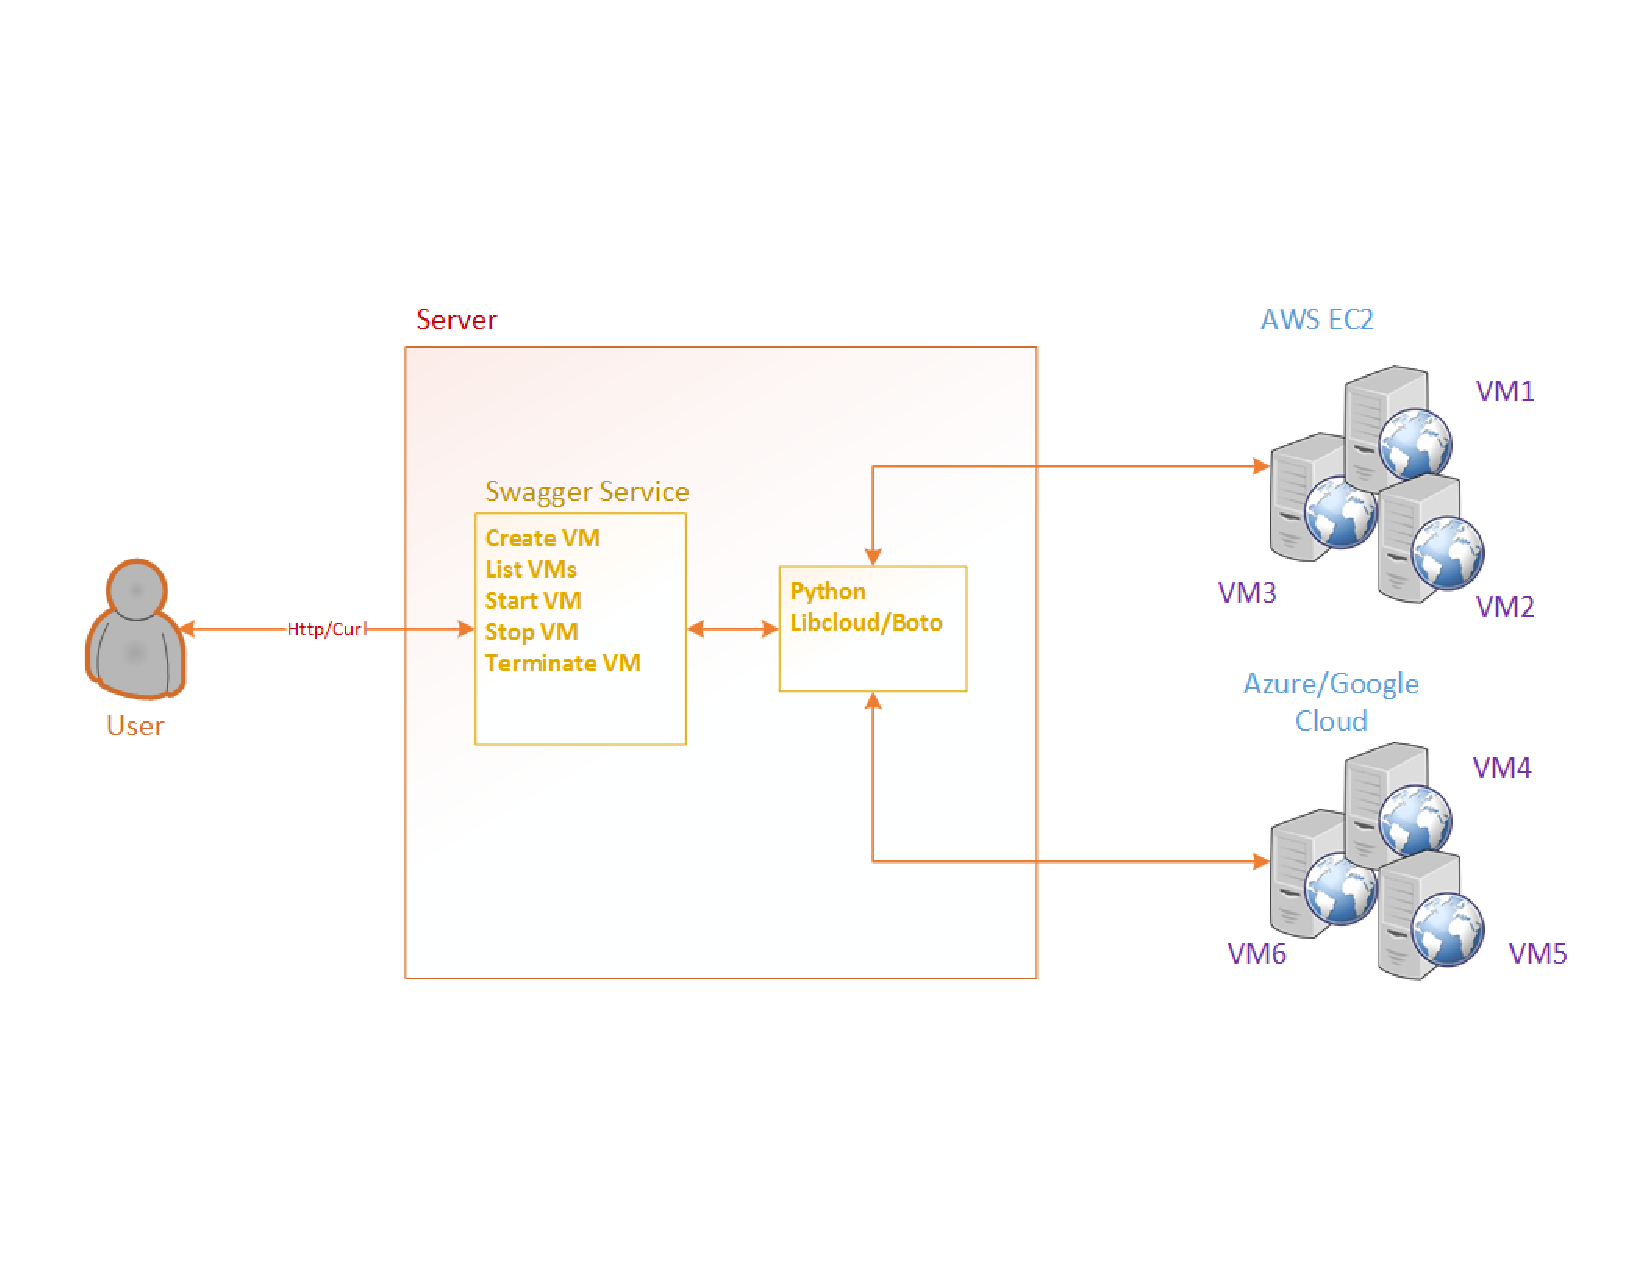
\includegraphics[width=\columnwidth]{images/proj-arch.pdf}
  \caption{Project Architecture}\label{F:arch}
\end{figure}

\section{Literature Review}

The National Institute of Standards and Technology defines cloud  portability as ``data 
that can be moved from one cloud system to another and that  applications can be ported 
and run on different  cloud systems at an  acceptable cost.''~\cite{hid-sp18-518-NIST-291} 
The concept of portability can be extended to encompass the full application stack from
the web service to the underlying hardware itself. Portability can also simply mean the 
ability to ensure high availability where you only are looking to protect against one 
cloud provider being a single point of faiure.

In NIST Special Publication 500-293, the United States governement has
defined a strategic roadmap that includes ten formal recommendations
for all cloud usage. Out of the ten requirements, eight of them
reference portability and interoperability. The Standards Acceleration
to Jumpstart the Adoption of Cloud Computing (SAJACC) is an initiative
under the guidance of NIST 500-293 that is to define ``qualitative
testing of specifications against interoperability, security, and
portability requirements.''~\cite{hid-sp18-518-NIST-293}

To define portability further, we have to differentiate the tiers of cloud service and 
where portability may be needed. Cloud providers have generally grouped service into the
following four types.

\begin{itemize}
\item
  Infrastructure as a Service \- IaaS
\item
  Platform as a Service \- PaaS
\item
  Software as a Service \- SaaS
\item
  Functions as a Service \- FaaS
\end{itemize}

Each grouping has dependencies that can make portability more difficult. For example, AWS
Lamba, which is a FaaS solution, is highly specialized and the APIs in use are specific to
that vendor. While solutions like libcloud and boto attempt to include all providers, the 
speed of the market makes it challenging for portability libraries to include the latest 
and great cloud provider offerings.~\cite{hid-sp18-518-LibCloud} Another dependency is 
the complexity of what needs to be ported. IaaS is the closest cloud offering to 
bare-metal and dependencies for hardware-specific requirements are not a consideration 
for most portability offerings. As the adoption of containers and functions increases, 
legacy implementations of cloud solutions that leveraged IaaS will be more difficult to 
port over. 

The work by the Irish Centre for Cloud Computing provided a ``qualitative  comparative  
of current  open-source  IaaS frameworks'' which is in contrast to vendor offerings which
tend to lack in portability~\cite{hid-sp18-518-Comp-study}. The study was limited to the
five top open-source providers of IaaS and the derived outcome of the comparison was a 
breakdown over twenty categories that included portability to vendor IaaS. The summary
was that each solution is tailored towards a specific need and while portability is
possible, there are other challenges that are considered when choosing when and which
of many cloud providers you will end up using.

The research by Kostoska, Gusev and Ristov further highlights the
challenges with portability, open-source and standards. The
researchers were ``motivated by several open research questions about
cloud solutions, such as how to wisely choose a cloud host for
services and how to change the cloud provider in an easy
manner.''\cite{hid-sp18-518-Kostoska-Gusev-Ristov} The paper
stipulates that not only is it difficult to choose which cloud
provider to use but that the community of cloud providers and what
differentiates them continues to grow. The work concludes that no
standard exists and their own efforts are only to ``offer a
possibility for a documented service exchange.''

An interesting example of where multiple private sector providers can ensure 
interoperability is illustrated by Wired journalist Joe Weinman. In his writings, he
expresses how air travel is easy for a consumer to determine where to fly out of, how
to get through security, and to have confidence their bags will arrive. The history of
aviation is one of consolidation and resistance to standards yet the market ultimately 
did accept some level of standardization.~\cite{hid-sp18-518-Wired} Weinman concludes 
with ``The Internet took decades to go from a vision of packet switching to where it is 
today.  Between the IEEE, industry, and academia, one can hope that the vision of an 
Intercloud is now getting the attention it deserves.''

In summary, multiple efforts by government and academia are encouraging standardization. 
For cloud providers to capture the market opportunity of Federal, State and local 
institutions, they will be encouraged to comply with the newly developed standards. The 
counter is that private sector will continue to encourage specialization and consumer
demand continues to show exponential growth. As Weinman states, the Internet is now a 
blend of decades of collaboration, incentives and mistakes and cloud portability will
likely be the same.

\section{Background on LibCloud}

The concept of LibCloud began in 2009 to address the growing challenge of API diversity
between the dozens of cloud providers. The effort eventually became a top level Apache 
project in 2011. LicCloud provides support for the three Cloud providers we tested, 
Amazon Web Services, Microsoft Azure and Google Cloud and also supports dozens more.

The solution breaks down support between seven primary aspects, which are Compute, 
Storage, Key Pair Management, Load Balancing, Container, Backups, and DNS. The support
for each aspect varies depending on the native support by the provider and the project
status. Another important consideration is region support which is typically restrained
to the primary region. This may limit the usefulness for projects that leverage cloud
resources globally.

Each aspect has a varying degree of functions available that also may not be fully 
available to leverage. For example, the supported methods for Compute are fully 
implemented for EC2 and Azure Virtual Machines yet the deploy node method is not yet
available for Google Compute Engine. An example that demonstrates the challenge with
migrating to a newer service provider is key management. Amazon EC2 fully supports all 
methods for key management yet Azure and Google Cloud Engine do not support even one.

Another challenge is that each cloud provider does not offer a testing platform for the
use of LibCloud. To test the use of the APIs, you will have to leverage production 
services to determine the solution works. We leveraged free trials to develop the use 
of libcloud which is suboptimatal for long-term development.

\section{Methodology}

Python libraries exist now that help you abstract your project from  your cloud provider. 
This may be important if you think you may need to use multiple cloud providers or if you 
want to ensure you take steps to avoid provider lock-in. There are multiple providers in 
this space and one of them is Apache Libcloud~\cite{hid-sp18-518-LibCloud} To put it 
simply, this library allows you to code simple resource  management that is independent 
of cloud provider specific API calls.

Our research is intended to prove that their is significant value to leveraging 
frameworks that provide portability. By comparing the native porting of an application to
a defined RESTful API, we theorize the porting of a service between cloud providers will
be more efficient. The combination of open-source portability python libraries, the speed 
of Swagger, and the standardization of REST will be a combination that will drastically
improve portability.

The Cloud Security Council has broken cloud portability into five measurable aspects of 
instruction, syntactic, metadata, behavior and policy. We will leverage the instruction
aspect, where the correct application instructions are followed when ported, and the 
syntactic facet where porting between providers is transparent to the end user. This
implies our testing is more closely aligned with real-world adoption but assumes aspects
like policy are left unattended.~\cite{hid-sp18-518-Cloud-Council}

The instruction facet looks to assess whether the intended target that is being ported to 
is capable of ``understanding and executing the instructions contained in the executable 
artifacts of the application.''~\cite{hid-sp18-518-Cloud-Council} This is a strong 
consideration if you are running code that depends on an underlying runtime environment, 
especially if it depends on a specific environment such as the difference between Java 
Runtime 7 or 8. When the porting is poorly executed, it may result in execution failures, 
poor performance or even worse, the instruction appears to run yet gives inaccurate 
results that must be found by regression testing.

The syntactic element looks to identify the ease of the solution to alleviate knowledge 
of the underlying syntax for the cloud provider API or needing to manually convert 
different unit sizes. This is salient when providers may use custom naming conventions or 
if the cloud provider expects steps to be executed in a specific fashion. This is also 
important at higher abstraction layers such as the application data itself, where the 
``PaaS service may provide instances of databases ready-to-use, in which
case the actual databases provided may be sensitive to the data syntax of the 
customer data.''~\cite{hid-sp18-518-Cloud-Council} The syntactic element is also where
we will highlight issues for cross-platform support in instances where the target 
provider either does not have API support or libcloud does not support yet.

\section{Discussion}

To experiment, we leveraged the following resources.

\begin{itemize}
    \item
    Swagger development to design/build API services for UI
  \item
    Python development to leverage libcloud
  \item
    Amazon Web Services, Azure, and Google Cloud
  \item
    Swagger API documentation
  \end{itemize}

To reflect on the three cloud providers chosen, the results were expected to skew towards
the strengths and weaknesses of each provider. AWS is considered the most mature provider 
with a very deep API offering where solutions like Azure are making progress. 
Alternatively, Data Motion states ``Google developed the Kubernetes standard that AWS and 
Azure now offer and GCP specializes in high compute offerings like Big Data, analytics and 
machine learning.''\cite{hid-sp18-518-DataMotion}

\begin{figure}[!ht]
  \centering
  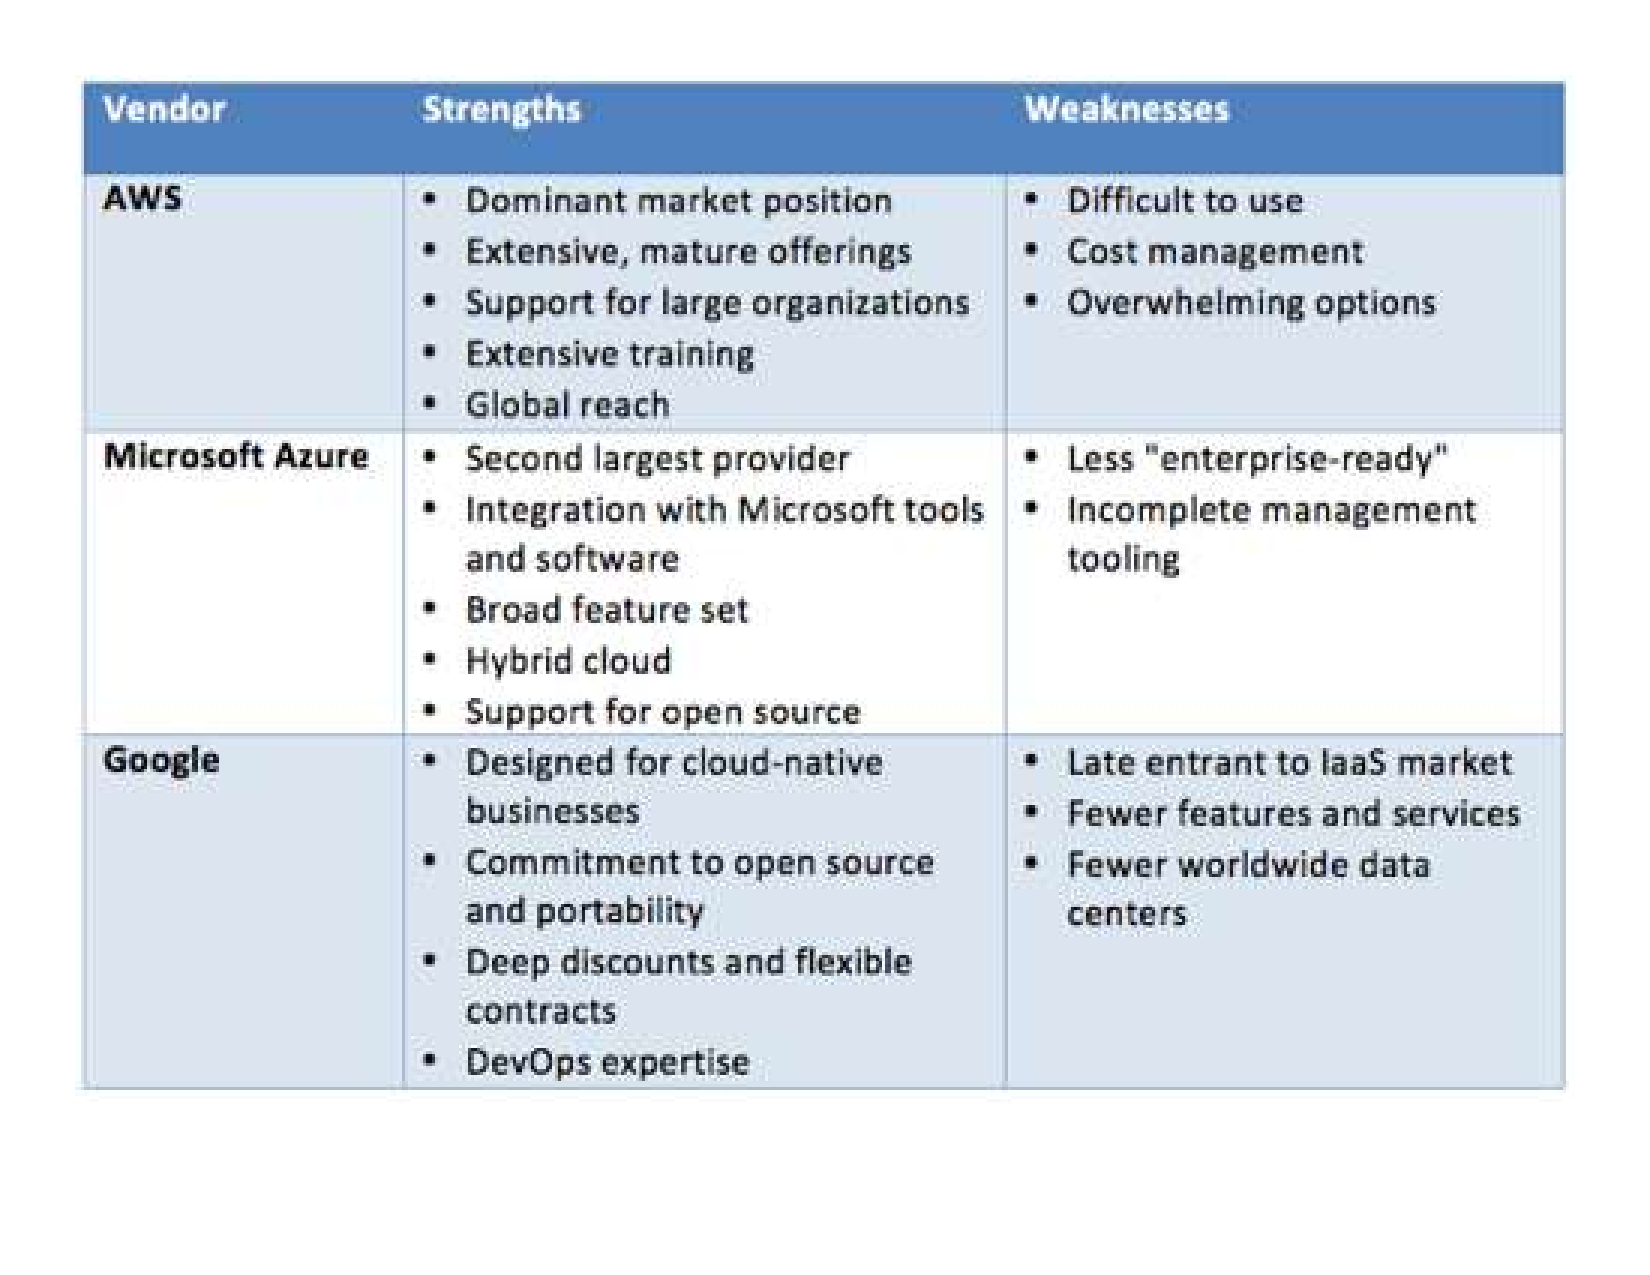
\includegraphics[width=\columnwidth]{images/aws-azure-google.pdf}
  \caption{Provider Comparison}\label{F:comparison}
\end{figure}

To determine the effectiveness, we have chosen to measure the cycle time on porting a 
solution without libcloud to two alternatives, leveraging native libcloud only and then 
our RESTful implementation of libcloud. Additionally, we will measure the lead time 
metrics on using a RESTful API compared to the command line python libraries to determine
if removing the expectation for portability can improve application development speed.

\subsection{Use of libcloud library with Python}

To use the libcloud library in your python environment, you install the apache-libcloud 
package using the Python package management system, pip. Libcloud currently supports Python
versions 2.5, 2.6, 2.7 and Python 3. To use libcloud as a library,
leverage Python and import libcloud like any other library. A useful feature to use in 
Python is the help function which will provide you a simple 
manual on further use of libcloud.

We leveraged libcloud to configure and manage EC2 in AWS. We first needed to configure 
credentials for an active cloud provider account and then configured libcloud provider 
to use that account. To be able to access AWS S3 from libcloud, we need the access key 
to be specified in the call. An access key can be setup on AWS console by navigating to 
My Security credentials, Encryption Keys, and then Access Keys.Next, local variables 
were defined to store the credentials to be used. Once that was set up, we defined the EC2 
driver with our region preference, which was AWS us-east-1, the most full featured region. 
This is because there are additional tasks that must be taken with SSH keys. We used our 
browser to review EC2 and finalize the setup.
 
\section{Results}

Comparison of command line tools to Python libraries libcloud and boto

\section{Summary}

\begin{acks}

  The authors would like to thank Dr.~Gregor~von~Laszewski for his
  support and suggestions to write this paper.

\end{acks}

\bibliographystyle{ACM-Reference-Format}
\bibliography{report} 

